\documentclass[8pt,a4paper,compress]{beamer}

\usepackage{/home/siyer/lib/slides}

\title{Modules and Clients}
\date{}

\begin{document}
\begin{frame}
\vfill
\titlepage
\end{frame}

\begin{frame}
\frametitle{Outline}
\tableofcontents
\end{frame}

\section{Using Functions in Other Programs}
\begin{frame}[fragile]
\pause

Using modular programming we can not only divide a program into functions, but also keep them in different files

\pause
\bigskip

We distinguish between two types of Python programs
\begin{itemize}
\item A module contains functions that are available for use by other programs

\item A client is a program that makes use of a function in a module
\end{itemize}

\pause
\bigskip

Five steps involved in creating and using modules
\begin{enumerate}
\item In the client, import the module

\item In the client, qualify function calls to the module

\item In the module, compose a test client

\item In the module, eliminate arbitrary global code

\item Make the module accessible to the client
\end{enumerate}

\pause
\bigskip

Modular programming enables us to independently develop and debug functions for an application and then utilize them at any later time
\end{frame}

\section{Modular Programming Abstractions}
\begin{frame}[fragile]
\pause
User-defined modules are files that each contain a set of related functions for use by other programs

\pause
\bigskip

We use three abstractions to manage the process of developing user-defined modules
\begin{enumerate}
\item Application programming interfaces (APIs)
\begin{center}
\begin{tabular}{cc}
function & description \\ \hline
\lstinline$pdf(x, mu, sigma)$ & Gaussian pdf \\
\lstinline$cdf(z, mu, sigma)$ & Gaussian cdf \\
\end{tabular} 
\end{center}

\item Clients
\begin{lstlisting}[language=Python]
percent = gaussian.cdf(score, mu, sigma)
\end{lstlisting}

\item Implementations
\begin{lstlisting}[language=Python]
def pdf(x, mu = 0.0, sigma = 1.0):
    ...
    
def cdf(z, mu = 0.0, sigma = 1.0):
    ...
\end{lstlisting}
\end{enumerate}
\end{frame}

\begin{frame}[fragile]
\pause

A library is a collection of related modules

\pause
\bigskip

For example, NumPy is a library for scientific computing

\pause
\bigskip

A private function, having its name start with an underscore by convention, is a helper function that is not intended to be called directly by clients
\begin{lstlisting}[language=Python]
def _phi(x):
    return math.exp(- x * x / 2.0) / math.sqrt(2 * math.pi)
    
def phi(x, mu = 0.0, sigma = 1.0):
    return _phi((x - mu) / sigma) / sigma
\end{lstlisting}

\pause
\bigskip

Documentation for modules and their functions is provided by embedding the documentaion string in triple quotes
\begin{lstlisting}[language=Python]
"""
stdrandom.py

The stdrandom module defines functions related to pseudo-random numbers.
"""
...
def uniformInt(lo, hi):
    """
    Return an integer chosen uniformly from the range [lo, hi).
    """
    return random.randrange(lo, hi)
...
\end{lstlisting}
\end{frame}

\section{Random Numbers}
\begin{frame}[fragile]
\pause

API for \lstinline{stdrandom} module
\begin{center}
\begin{tabular}{cc}
function & description \\ \hline
\lstinline$seed(i)$ & seed the random number generator with integer $i$ \\
\lstinline$uniformInt(lo, hi)$ & uniform random integer in the range $[lo, hi)$ \\
\lstinline$uniformFloat(lo, hi)$ & uniform random float in the range $[lo, hi)$ \\
\lstinline$bernoulli(p)$ & \lstinline$True$ with probability $p$ (defaults to 0.5) \\
\lstinline$binomial(n, p)$ & \makecell{number of heads in $n$ coin flips, each of which is \\ heads with probability $p$ (defaults to 0.5)} \\
\lstinline$gaussian(mu, sigma)$ &  \makecell{normal, mean $mu$ (defaults to 0), \\ standard deviation $sigma$ (defaults to 1)} \\
\lstinline$discrete(a)$ & $i$ with probability proportional to $a[i]$ \\
\lstinline$shuffle(a)$ & randomly shuffle the list $a$ \\
\lstinline$exp(lambd)$ & a float from an exponential distribution with rate $lambd$ 
\end{tabular} 
\end{center}
\end{frame}

\begin{frame}[fragile]
\pause

\begin{framed}
\tiny stdrandom\_client.py: Accept integer $trials$ as a command-line argument. Plot $trials$ number of $(x, y)$ points to standard draw, where $x$ and $y$ are drawn from a Gaussian distribution.
\end{framed}

\begin{lstlisting}[language=Python]
import stddraw
import stdrandom
import sys

trials = int(sys.argv[1])
stddraw.setPenRadius(0.0)
for i in range(trials):
    x = stdrandom.gaussian(0.5, 0.2)
    y = stdrandom.gaussian(0.5, 0.2)
    stddraw.point(x, y)
stddraw.show()
\end{lstlisting}

\pause

\begin{minipage}{160pt}
\begin{lstlisting}[language={}]
$ python3 stdrandom_client.py 100000
\end{lstlisting}
\end{minipage}%
\begin{minipage}{140pt}
\hfill \visible<3->{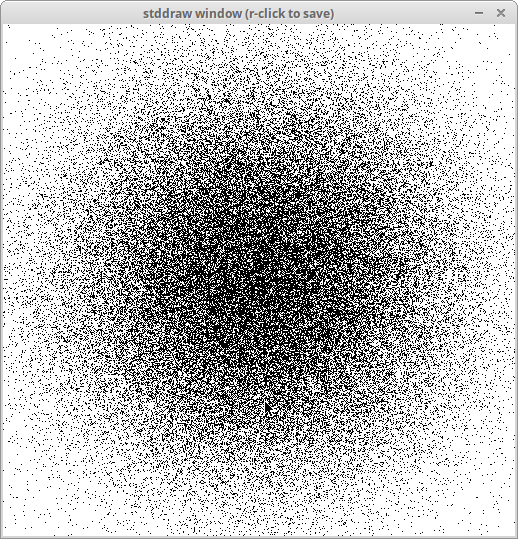
\includegraphics[scale=0.17]{figures/stdrandom_client.png}}
\end{minipage}
\end{frame}

\begin{frame}[fragile]
\pause

\begin{framed}
\tiny stdrandom.py: Random number module that defines functions related to pseudo-random numbers.
\end{framed}

\begin{lstlisting}[language=Python]
import random
import math

def seed(i = None):
    random.seed(i)

def uniformInt(lo, hi):
    return random.randrange(lo, hi)
    
def uniformFloat(lo, hi):
    return random.uniform(lo, hi)

def bernoulli(p = 0.5):
    return random.random() < p

def binomial(n, p = 0.5):
    heads = 0
    for i in range(n):
        if bernoulli(p):
            heads += 1
    return heads
    
def gaussian(mu = 0.0, sigma = 1.0):
    return random.gauss(mu, sigma)
\end{lstlisting}
\end{frame}

\begin{frame}[fragile]
\pause

\begin{lstlisting}[language=Python]
def discrete(a):
    r = uniformFloat(0.0, sum(a))
    subtotal = 0.0
    for i in range(len(a)):
        subtotal += a[i]
        if subtotal > r:
            return i

def shuffle(a):
    random.shuffle(a)

def exp(lambd):
    return -math.log(1 - random.random()) / lambd
    
def _main():
    import sys
    import stdio
    seed(1)
    n = int(sys.argv[1])
    for i in range(n):
        stdio.writef(' %2d '   , uniformInt(10, 100))
        stdio.writef('%8.5f '  , uniformFloat(10.0, 99.0))
        stdio.writef('%5s '    , bernoulli())
        stdio.writef('%5s '    , binomial(100, .5))
        stdio.writef('%7.5f '  , gaussian(9.0, .2))
        stdio.writef('%2d '    , discrete([.5, .3, .1, .1]))
        stdio.writeln()

if __name__ == '__main__':
    _main()
\end{lstlisting}
\end{frame}

\section{List Processing}
\begin{frame}[fragile]
\pause

API for \lstinline{stdarray} module
\begin{center}
\begin{tabular}{cc}
function & description \\ \hline
\lstinline$create1D(n, val)$ & list of length $n$, each element initialized to $val$ \\
\lstinline$create2D(m, n, val)$ & $m$-by-$n$ list, each element initialized to $val$ \\
\lstinline$write1D(a)$ & write list $a$ to standard output \\
\lstinline$write2D(a)$ & write two-dimensional list $a$ to standard output \\
\lstinline$readInt1D()$ & list of integers, read from standard input \\
\lstinline$readInt2D()$ & two-dimensional list of integers, read from standard input \\
\lstinline$readFloat1D()$ & list of floats, read from standard input \\
\lstinline$readFloat2D()$ & two-dimensional list of floats, read from standard input \\
\lstinline$readBool1D()$ & list of booleans, read from standard input \\
\lstinline$readBool2D()$ & two-dimensional list of booleans, read from standard input
\end{tabular} 
\end{center}
\end{frame}

\begin{frame}[fragile]
\pause

\begin{framed}
\tiny ifs.py: Accept integer $n$ as a command-line argument. Read a $1$-by-$m$ vector (probabilities) and two $m$-by-$3$ matrices (coefficients for updating $x$ and $y$, respectively) from standard input. Plot the results as a set of $n$ points to standard draw.
\end{framed}

\begin{lstlisting}[language=Python]
import stdarray
import stddraw
import stdrandom
import sys

def main():
    n = int(sys.argv[1])
    dist = stdarray.readFloat1D()
    cx = stdarray.readFloat2D()
    cy = stdarray.readFloat2D()
    x = 0.0
    y = 0.0
    stddraw.setPenRadius(0.0)
    for i in range(n):
        r = stdrandom.discrete(dist)
        x0 = cx[r][0] * x + cx[r][1] * y + cx[r][2]
        y0 = cy[r][0] * x + cy[r][1] * y + cy[r][2]
        x = x0
        y = y0
        stddraw.point(x, y)
    stddraw.show()

if __name__ == '__main__':
    main()
\end{lstlisting}
\end{frame}

\begin{frame}[fragile]
\pause

Sierpinski triangle

\begin{minipage}{160pt}
\begin{lstlisting}[language={}]
$ more sierpinski.txt
3   
  .33 .33 .34 
3 3 
  .50 .00 .00 
  .50 .00 .50 
  .50 .00 .25 
3 3 
  .00 .50 .00 
  .00 .50 .00 
  .00 .50 .433 
$ python3 ifs.py 20000 < sierpinski.txt
\end{lstlisting}
\end{minipage}%
\begin{minipage}{140pt}
\begin{center}
\hfill \visible<2->{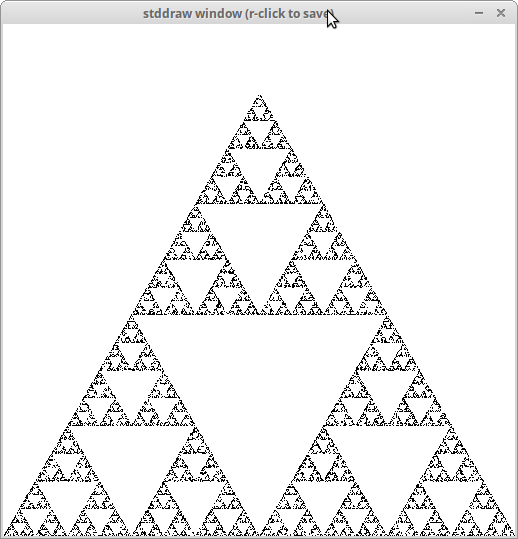
\includegraphics[scale=0.17]{figures/sierpinski.png}}
\end{center}
\end{minipage}

\pause
\bigskip

Barnsley fern

\begin{minipage}{160pt}
\begin{lstlisting}[language={}]
$ more barnsley.txt
4
   0.01  0.85  0.07  0.07
4 3
   0.00  0.00  0.500
   0.85  0.04  0.075
   0.20 -0.26  0.400
  -0.15  0.28  0.575
4 3
   0.00  0.16  0.000
  -0.04  0.85  0.180
   0.23  0.22  0.045
   0.26  0.24 -0.086
$ python3 ifs.py 20000 < barnsley.txt
\end{lstlisting}
\end{minipage}%
\begin{minipage}{140pt}
\begin{center}
\hfill \visible<3->{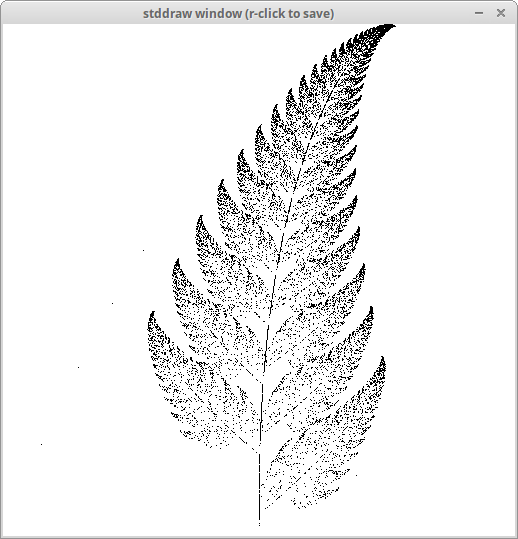
\includegraphics[scale=0.17]{figures/barnsley.png}}
\end{center}
\end{minipage}
\end{frame}

\begin{frame}[fragile]
\pause

\begin{framed}
\tiny stdarray.py: List module that defines functions related to creating, reading, and writing one- and two-dimensional lists.
\end{framed}

\begin{lstlisting}[language=Python]
import stdio

def create1D(length, value=None):
    return [value] * length

def create2D(rowCount, colCount, value=None):
    a = [None] * rowCount
    for row in range(rowCount):
        a[row] = [value] * colCount
    return a

def write1D(a):
    length = len(a)
    stdio.writeln(length)
    for i in range(length):
        element = a[i]
        if isinstance(element, bool):
            if element == True:
                stdio.write(1)
            else:
                stdio.write(0) 
        else:
            stdio.write(element)
        stdio.write(' ')
    stdio.writeln()
\end{lstlisting}
\end{frame}

\begin{frame}[fragile]
\pause

\begin{lstlisting}[language=Python]
def write2D(a):
    rowCount = len(a)
    colCount = len(a[0])
    stdio.writeln(str(rowCount) + ' ' + str(colCount))
    for row in range(rowCount):
        for col in range(colCount):
            element = a[row][col]
            if isinstance(element, bool):
                if element == True:
                    stdio.write(1)
                else:
                    stdio.write(0)
            else:
                stdio.write(element)
            stdio.write(' ')
        stdio.writeln()

def readInt1D():
    count = stdio.readInt()
    a = create1D(count, None)
    for i in range(count):
        a[i] = stdio.readInt()
    return a

def readInt2D():
    rowCount = stdio.readInt()
    colCount = stdio.readInt()
    a = create2D(rowCount, colCount, 0)
    for row in range(rowCount):
        for col in range(colCount):
            a[row][col] = stdio.readInt()
    return a
\end{lstlisting}
\end{frame}

\begin{frame}[fragile]
\pause

\begin{lstlisting}[language=Python]
def readFloat1D():
    count = stdio.readInt()
    a = create1D(count, None)
    for i in range(count):
        a[i] = stdio.readFloat()
    return a

def readFloat2D():
    rowCount = stdio.readInt()
    colCount = stdio.readInt()
    a = create2D(rowCount, colCount, 0.0)
    for row in range(rowCount):
        for col in range(colCount):
            a[row][col] = stdio.readFloat()
    return a

def readBool1D():
    count = stdio.readInt()
    a = create1D(count, None)
    for i in range(count):
        a[i] = stdio.readBool()
    return a
\end{lstlisting}
\end{frame}


\begin{frame}[fragile]
\pause

\begin{lstlisting}[language=Python]
def readBool2D():
    rowCount = stdio.readInt()
    colCount = stdio.readInt()
    a = create2D(rowCount, colCount, False)
    for row in range(rowCount):
        for col in range(colCount):
            a[row][col] = stdio.readBool()
    return a

def _main():
    write2D(readFloat2D())
    write2D(readBool2D())

if __name__ == '__main__':
    _main()
\end{lstlisting}
\end{frame}

\section{Standard Statistics}
\begin{frame}[fragile]
\pause

API for \lstinline{stdstats} module
\begin{center}
\begin{tabular}{cc}
function & description \\ \hline
\lstinline$mean(a)$ & average of the values in the numeric list $a$ \\
\lstinline$var(a)$ & sample variance of the values in the numeric list $a$ \\
\lstinline$stddev(a)$ & sample standard deviation of the values in the numeric list $a$ \\
\lstinline$median(a)$ & median of the values in the numeric list $a$ \\
\lstinline$plotPoints(a)$ & point plot of the values in the numeric list $a$ \\
\lstinline$plotLines(a)$ & line plot of the values in the numeric list $a$ \\
\lstinline$plotBars(a)$ & bar plot of the values in the numeric list $a$
\end{tabular} 
\end{center}
\end{frame}

\begin{frame}[fragile]
\pause

\begin{framed}
\tiny bernoulli.py: Accept integers $n$ and $trials$ as command-line arguments. Perform $trials$ experiments, each of which counts the number of heads found when a fair coin is flipped $n$ times. Then draw the results to standard draw. 
\end{framed}

\begin{lstlisting}[language=Python]
import gaussian
import math
import stdarray
import stddraw
import stdrandom
import stdstats
import sys

def main():
    n = int(sys.argv[1])
    trials = int(sys.argv[2])
    freq = stdarray.create1D(n + 1, 0)
    for t in range(trials):
        heads = stdrandom.binomial(n, 0.5)
        freq[heads] += 1
    norm = stdarray.create1D(n + 1, 0.0)
    for i in range(n + 1):
        norm[i] = 1.0 * freq[i] / trials
    phi = stdarray.create1D(n + 1, 0.0)
    stddev = math.sqrt(n) / 2.0
    for i in range(n + 1):
        phi[i] = gaussian.pdf(i, n / 2.0, stddev)
    stddraw.setCanvasSize(1000, 400)
    stddraw.setYscale(0, 1.1 * max(max(norm), max(phi)))
    stdstats.plotBars(norm)
    stdstats.plotLines(phi)
    stddraw.show()

if __name__ == '__main__':
    main()
\end{lstlisting}
\end{frame}

\begin{frame}[fragile]
\pause

\begin{minipage}{160pt}
\begin{lstlisting}[language={}]
$ python3 bernoulli.py 20 100000
\end{lstlisting}
\end{minipage}%
\begin{minipage}{140pt}
\hfill \visible<2->{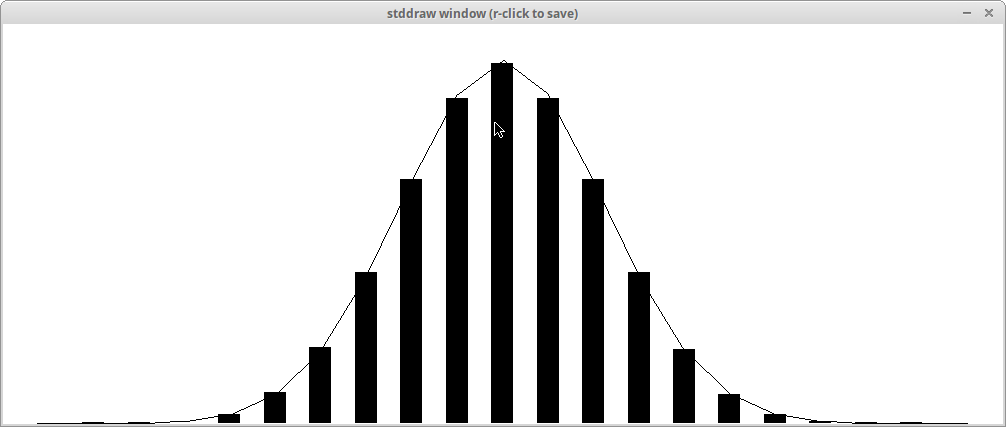
\includegraphics[scale=0.12]{figures/bernoulli.png}}
\end{minipage}
\end{frame}

\begin{frame}[fragile]
\pause

\begin{framed}
\tiny stdstats.py: Statistics module that defines functions related to statistical analysis and graphical data display.
\end{framed}

\begin{lstlisting}[language=Python]
import math
import stddraw

def mean(a):
    return sum(a) / len(a)

def var(a):
    mu = mean(a)
    total = 0.0
    for x in a:
        total += (x - mu) * (x - mu)
    return total / (len(a) - 1)

def stddev(a):
    return math.sqrt(var(a))

def median(a):
    b = sorted(a)
    length = len(b)
    if length % 2 == 1:
        return b[length // 2]
    else:
        return (b[length // 2 - 1] + b[length // 2]) / 2
\end{lstlisting}
\end{frame}

\begin{frame}[fragile]
\pause

\begin{lstlisting}[language=Python]
def plotPoints(a):
    n = len(a)
    stddraw.setXscale(-1, n)
    stddraw.setPenRadius(1.0 / (3.0 * n))
    for i in range(n):
        stddraw.point(i, a[i])

def plotLines(a):
    n = len(a)
    stddraw.setXscale(-1, n)
    stddraw.setPenRadius(0.0)
    for i in range(1, n):
        stddraw.line(i - 1, a[i - 1], i, a[i])

def plotBars(a):
    n = len(a)
    stddraw.setXscale(-1, n)
    for i in range(n):
        stddraw.filledRectangle(i - 0.25, 0.0, 0.5, a[i])

def _main():
    import stdarray
    import stdio
    a = stdarray.readFloat1D()
    stdio.writef('      mean %7.3f\n', mean(a))
    stdio.writef('   std dev %7.3f\n', stddev(a))
    stdio.writef('    median %7.3f\n', median(a))

if __name__ == '__main__':
    _main()
\end{lstlisting}
\end{frame}

\end{document}
